\chapter{Introduction}

%Allgemeines über Gebirgsmechanik
\begin{quote} 
\textit{``Rock fails because the stresses overcome the rockmass strength.''} \\
\autocite[2.13]{canada96}
\end{quote} 
This the basic principle behind rock mechanics. It's not possible to change the inherent strength of the rock, only to enhance it through rock support. \autocite{Hoek80} %The stresses are caused by forces that are applied to the rock mass. 

%%%%%%%%%%%%%%%% difference between static and dynamic loading
%TO DO put something here!

%Usually rock support has to withstand static load. The difference between static and dynamic load is best described by \textcite{Timo56} who states that ``Statics deals with the conditions of bodies acted upon by forces'' whereas dynamics is defined as ``the relationship between the kind of motion of a particle and the forces producing it''. From this definition it becomes obvious that dynamic load is connected to movement, whereas static load is motionless. Of course, there is no pure static load in mining, rock creeps and deforms, therefore it´s preferable to refer to this state as quasi-static.


There are two types of stress inside the rock mass: quasi - static stress and dynamic stress.
Dynamic stresses can be caused by seismic events. An easy way to distinguish between static and dynamic stresses is the strain rate  (\( \dot{\varepsilon} \)).  \( \dot{\varepsilon} \) means the change in length per second. After \textcite{strain04}: $\dot{\varepsilon} = \int \frac{l(t)}{l_0} dt  $. With $l(t)$ as the size at a given time and $l_0$ as the size at $t=0$. \textcite[3]{ali2002} stated that static load causes \( \dot{\varepsilon} \) of approximately $ 10^{-5}~\text{s}^{-1} $. 
Compared to that, dynamic loading, specifically seismic events, can cause \(\dot{\varepsilon} = 5 * 10^{-3}~\text{s}^{-1}~ \dot{\varepsilon}\) while blasting can reach up to can cause \(\dot{\varepsilon} = 10^{3}~\text{s}^{-1}~\). The strain rate during seismic events is much higher than the strain rate under static loading conditions. 
\textcite[6]{reinhardt82} stated that a seismic event may cause loading rates of up to 100 \(\frac{\text{N}}{\text{mm}^\text{2}}*\text{ms}\).  %Seismic events can be characterized by a several parameters including: amplitude of the the seismic wave, released energy and distance from the observer. These parameters influence the tensions inside of the rock and the demands on the rock support. 
%Type of seismic event
\section{Different Types of Seismic Events}
\textcite[3]{player04} defined a seismic event as: "A release of built up strain energy." %from the formation of excavations that does not result in a fall of ground or yielding of ground control scheme
The released energy travels through the rock in the form of a wave. It possesses an amplitude and a frequency.
 According to \textcite{durrheim06} seismic events can be grouped in 3 categories according to their relation to mining activity:
 
 \begin{itemize}
     \item Natural
     \item Mining triggered
     \item Mining induced
 \end{itemize}
 
A natural earthquake is not caused or influenced by human activity.%, especially mining, in any way. 

A mining triggered earthquake only happens along a pre-existing fault. Mining activity triggers these events but is not the driving force.
%contributes only a small fraction of the observed energy. 
These events can happen at considerable distance to mining operations.

Mining induced events are directly caused by mining. Most of the observed energy stems directly from mining activities or mining related stresses. They often happen along pre-existing faults or create new ruptures. 

The resulting tensions in the rock mass depend
%The demands such an event puts on the rock mass are dependant 
The resulting tensions in the rock mass depend on several factors: the magnitude of the triggering seismic event, the rate at which it releases its energy and the distance from the hypocentre of the event. %as well as the properties of the rock in between hypocenter and excavation as well as directly around the excavation.
If the demands of the seismic event exceed the capabilities of the rock support, it will fail. A failure of the rock support and the associated consequences, such as ejected rock, are summarized under the term rockburst.
It is crucial to differentiate between the seismic event and the observed damage mechanism. \autocite{Kaiser12} \autocite[9]{Heal10}

%Damage mechanism
\section{Damage Mechanism}

%There are several different modes failure under of dynamic loading, they are in general combined under the term ``rockburst''. 
%\textcite{Hoek80} defines rockbursts as: ``Rockbursts are explosive rock failures which can occur when strong brittle rock is subjected to high stress.'' which is a very general definition focusing on rock mechanics. Most definitions put the different failure modes more into the foreground. For example 
%\Textcite[271]{Brady99} defines rockbursts: "A rockburst is the sudden displacement of rock, under seismic impulse, in the boundary of an excavation, causing substantial damage to it." 
%which only describes a very specific type of damage mechanism.
%\textcite{Brauner94} defines rockbursts as: ``Rockbursts are violent failures in the ground, breaking rock and expelling it into excavations.'' 
%On the other hand \textcite[582]{Obert67} provides following definition ``A rockburst is defined as any violent expulsion of rock from its surroundings, the phenomenon resulting from static stress exceeding the static strength of the rock'' This definition introduces another important factor: static stress. %With this definition in mind it becomes obvious that Static stress is necessary to cause dynamic loading. Though
\textcite[582]{Obert67} defined rockbursts as: 
 "any violent expulsion of rock from its surroundings, the phenomenon resulting from static stress exceeding the static strength of the rock''

High static stress and sufficiently brittle rock are needed to create rock bursts. \autocite[6]{Brauner94} \autocite[2.10]{canada96} Which is why Kiirunavaara Mine had only minor problems with rockbursts until the rock mass quality significantly increased at a depth of around 900 m. The reason for this increase is unclear. \autocite[4]{dahner12} %became significantly more brittle 
 Static stress in general increases with depth, that is why vulnerability to rockbursts is usually thought to increase with depth. \autocite[8]{Brauner94}

There are records of very deep mines which are seismically inactive as well as of rockbursts in open pit mines or at shallow depths. %Especially in Australia because of the high vertical stresses present in the ground. 
\autocite[584]{Obert67} Other factors than depth must also influence how burst prone ground is.
%Other factors also influence how burst prone the rock mass is. 
  %the magnitude of the triggering seismic event, the rate at which it releases its energy and the distance from the hypocenter of the event to the excavation. 
Rock properties like rock type, rock strength, joint fabric and rock brittleness influence the behavior of the rock. The stress distribution is influenced by the existence of geological structures, mining induced static stresses, the span of the excavation, the extraction ratio, the production rate, the  mine stiffness, the layout of the mine and if backfill is used, the properties of the backfill material.  \autocite[2.10]{canada96} \autocite[219]{Kaiser12} \autocite[8]{Brauner94} 


The level of the dynamic stress in the rock mass also depend on the seismic event itself.
%The amount of dynamic load that the rock mass has to take is also an important factor. 
%The amount of dynamic stresses inside the rock mass is also an important factor. 
As previously discussed the stresses caused by a seismic event can be roughly estimated from the released energy, the rate at which this energy is released and the distance from hypocenter. To describe the amount of energy released by a seismic event the Richter scale can be used.
But not all rockbursts are equal, they can take different forms depending on various factors.
%\textcite[8]{Brauner94} writes: 
%\begin{quote} 
%\textit{''Even though other factors remain equal, both frequency and severity [of rockbursts] increases with depth.  This, however is overshadowed by influences of the local mining geometry, mainly the vicinity of other excavations.''}
%\end{quote} 

%In general rockbursts are cause by seismic events, either of natural or artificial origin, built up of stress in the affected area or other mechanisms. \autocite[24]{Brauner94} %They can happen seemingly at random in the case of bulking.\autocite[2.4]{canada96} 

%failure modes

%``Rockburst'' is also an umbrella term for a range of different failure modes. 
% The term "rockbursts" is applied to a range of different failure modes.
\textcite{Ortlepp97Fracture} defined the following failure mechanisms:

\begin{itemize}
\item strain burst
\item buckling
\item face crush/pillar burst
\item shear rupture
\item fault-slip burst
\end{itemize}

Strain bursting is a result of low Richter Magnitudes, between -0,2 and 0 and takes the form of superficial spalling with violent ejection of fragments. 
Buckling is a result of Richter magnitudes between 0 and 1,5. Large slabs or rock are expulsed into the excavation.
Face crush / pillar burst is a result of Richter Magnitudes between 1 and 2,5. As the name implies rock is violently expulsed from the stope face or the pillar sides.
Shear rupture is a result of 2 to 3,5 on the Richter Scale. Shear fractures violently propagate through the intact rock mass. 
Fault-slip describes violent movement along an existing fault. It is a result of 2,5 to 5 magnitude on the Richter Scale.

Under the right conditions, rockbursts will inevitably happen. \autocite[4]{Heal10} That is why it is important to learn how to reduce their frequency and severity.


\section{Reducing the Frequency and Severity of Rockbursts}
%what to do against rockbursts?
Essential in reducing the frequency and severity of rockbursts is reducing the stresses in the rock mass. There is a plethora of possible measures that can be taken in advance, for example: changing or modifying mining sequence, mining geometry, mining method, excavation shape, location of drifts and ore passes, stope size and using backfill or changing the properties of the backfill material. \autocite[219]{Kaiser12} As the vulnerability to rockbursts increases with excavation span, 4-way intersections should be avoided where possible. \autocite[323]{Heal10}
If a small area is dangerously overstressed, destress drill and blasting can be used to actively reduce the likelihood of a rockburst. \autocite[219]{Kaiser12}
Human safety can be increased through usage of remotely operated equipment. \autocite[3]{Heal10}
But rockbursts are impossible to predict reliably. \autocite[4]{Heal10} \autocite[10]{durrheim06} Measures such as destress blasting bring immediate release of tensions. But make the ground more prone to rocksbursts in the future by weakening the rock mass and increasing the amount of loose rock that can be mobilized during a rockburst. \autocite[61]{Brauner94} For certain applications destress blasting is incredibly useful but it is currently not used in Kiirunavaara mine.

\chapter{Rock Support}
%Rock support
The last line of defense against rockbursts is rock support. It is often also the most effective. \autocite[323]{Heal10}

%The maxim of surface support design in the Kiirunavaara Mine so far was very heavily based on the first concept with ever increasing thicknesses of shotcrete being applied as previous support concepts fail or after cleaning up rockfalls. This game can not be played indefinitely though. \textcite[2.17]{canada96} states that: \begin{quote}\textit{"As the rockburst severity increases, the support will not be able to prevent initiation of the damage mechanism. An appropriate support system must however be able to survive the displacements associated with the rockburst and remain functional after the rockburst to hold and retain broken rock."}\end{quote} It seems probable that the Kiirunavaara Mine is at a crossroads. Ever increasing static load is requiring stronger and stronger support in order to keep the rock mass from unraveling, while in some places catastrophic failures can be observed. It may worthwhile to invest heavier in yielding rock support. At this point in time it might be feasible to consider using reinforced shotcrete instead of mesh being attached over shotcrete or maybe even to progress as far as isolated shotcrete panels, in order to allow large initial deformations before the shotcrete panels are "activated".

%As soon as shotcrete tears, its support function is heavily impaired at this point the load must be taken by the welded mesh almost single handedly. This poses the question if the heavy use of shotcrete at Kiirunavaara is really cost effective. As explained in \autoref{sec:rockbursts} the main requirements posed by the currently observed failure modes are: abilty to survive heavy displacement as well as strong reinforcement of the rock mass. Which is difficult to archieve at the same time.
%(FIND THE PICTURES!) there are some rockfalls, where it is obvious that just the shotcrete and a thin layer of rock has been affected, with minor to moderate bulking being the failure mode. It is probable that a more flexible support system might have been able to absorb the excess energy through deformation. 

Rock supports main functions after \textcite{canada96} are maintaining the integrity of surrounding excavation, retaining fractured rock and preventing excessive excavation deformation.

\textcite{canada96} defined two kinds of support elements:% which full the 3 main functions:
\begin{itemize}
\item reinforcement support
\item surface support
\end{itemize}

\begin{comment}
\begin{table}
    \centering
    \begin{tabular}{l l p{5cm}}
        \toprule
        Displacement  & Energy Demand  & Recommended Bolt\\
         \(mm\)  &  \(\rfrac{kJ}{m^2}\)  & \\
         \midrule
        < 50 & < 5 & Expansion shell rock bolt, Resin/cement steel rebar\\
        50 - 100 & 5 - 15 & Split Set, Swellex, Roofex, Yield-Lok\\
        100 - 200 & 15 - 25 & Swellex, D-Bolt, Conebolt, Roofex, Yield-Lok\\
        200 - 300 & 25 - 35 & Roofex, Conebolt, Garford \\
        > 300 & > 35 & Conebolt, Garford\\
         \bottomrule
    \end{tabular}
    \caption{bolt recommendations after \textcite[580]{Masoudi18}}
    \label{tab:bolt}
\end{table}


\begin{figure}
    \centering
    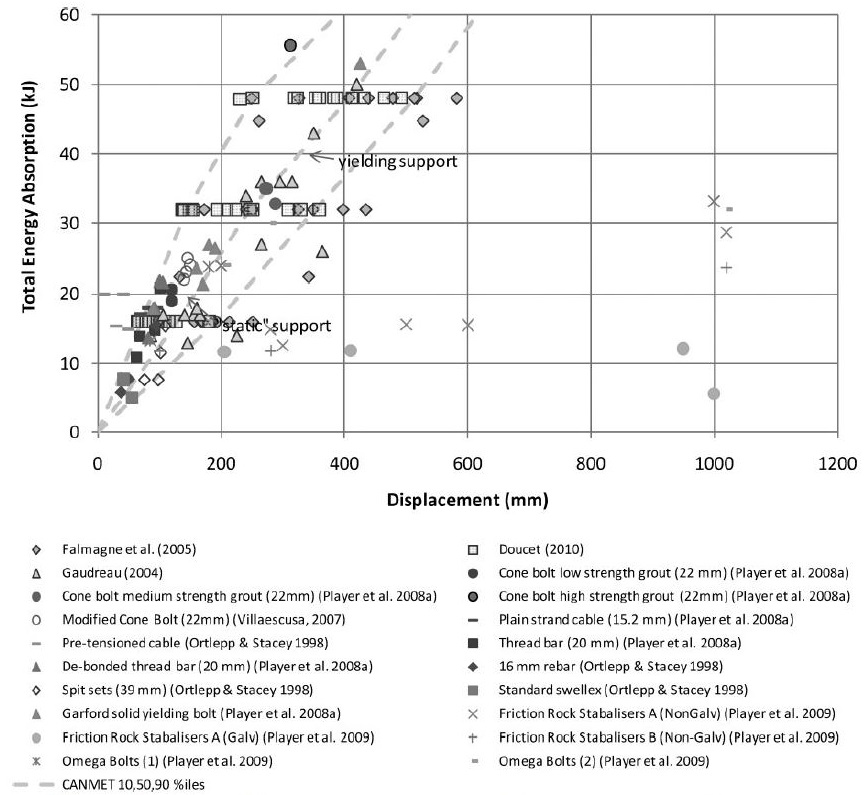
\includegraphics[width=0.9 \linewidth]{pics/potvin10_bolts.JPG}
    \caption{Compilation of the results various dynamic tests of bolts by \textcite{Potvin10}}
    \label{fig:potbol}
\end{figure}

\begin{figure}
    \centering
    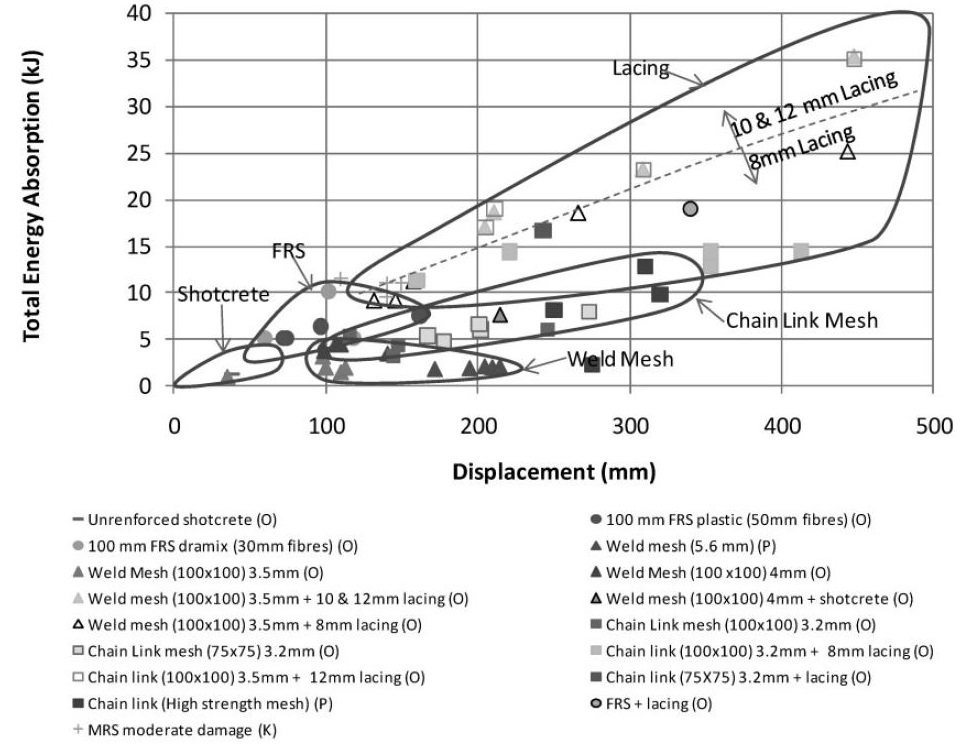
\includegraphics[width=0.9 \linewidth]{pics/potvin10_surface.JPG}
    \caption{compilation of the results various dynamic tests of surface support elements by \textcite{Potvin10}}
    \label{fig:potsur}
\end{figure}

\end{comment}
\section{Reinforcement Support}

%reinforcement support
\Textcite[312]{Brady99} defined reinforcement support as: "Means of conserving or improving the overall rock mass properties from within the rock mass".
%Reinforcement support elements have two functions: to increase the strength of the rock mass through reinforcement and to hold surface support elements in place. \autocite[2.16]{canada96} 
There are two design paradigms behind reinforcement support, depending on the rock conditions. One way is to contain deformations through anchoring large loose blocks to stable rock using widely spaced long bolts, which have to be able to survive large displacements. These long bolts directly secure large wedges and rocks to intact rock and high a high capacity to withstand deformations.
The other way is using tightly spaced short bolts with little displacement capabilities that deform with the rock. These short bolts confine highly fragmented rock mass around themselves and compact it into a "hard shell" around the excavation. \autocite[15]{guler01} These bolts do not deform themselves. They move with the rock that surrounds it.
Following the second paradigm it may be economical to install non-yielding bolts in burstprone ground. \autocite[6.23]{canada96}
%One kind of bolt may be used to satisfy both conditions but

In burst prone mines it often is more sensible to %have highly specialized bolts for try
have bolts for both of these tasks instead of just focusing on one. Especially in vulnerable areas such as intersections. Under quasi static loading conditions strength and cost are the deciding factors when designing a support system whereas burst prone ground requires high energy absorption capabilities and high displacement rates. %Nevertheless, it may be economical to install non-yielding bolts in burstprone ground. After a dynamic loading event, these bolts will have to be checked and possibly replaced. \autocite[6.23]{canada96} 
There are several kinds of bolts with varying suitability for use in burstprone mines. %, usually depending on their displacement and energy absorption capabilities. 
%Cone bolts, Swellex, Split Set bolts and debonded Cable bolts offer high displacement rates while at the same time having high peak load capacities. \autocite[4.14]{canada96} 
%In \autoref{tab:bolt} some bolt types and their dynamic capabilities are given. In \autoref{fig:potbol} the results of several dynamic tests of rock bolts are displayed. 

\begin{figure}
    \centering

\subcaptionbox{Square spacing of bolts}{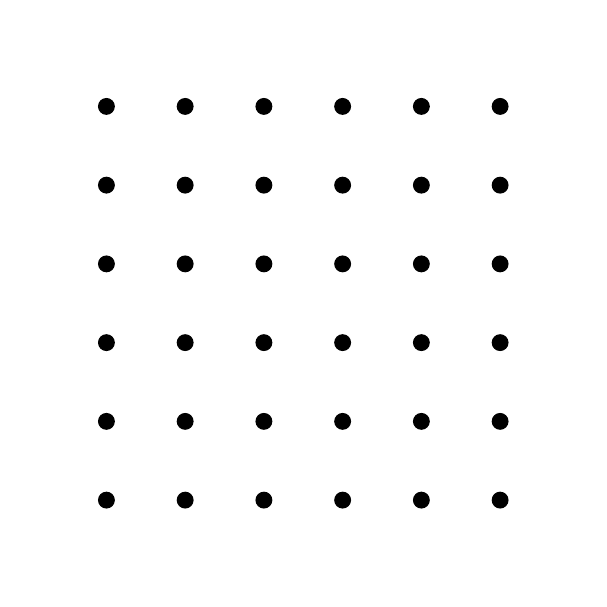
\begin{tikzpicture}
%SQUARE spacing
\path (0,0) -| (7,7);

\foreach \x in {1,2,...,6}{
\foreach \y in {1,2,...,6}{
\draw[fill = black] 
(0+\y,0+\x) circle [radius=0.1]
;}}

\end{tikzpicture}}
\subcaptionbox{Diamond spacing of bolts}{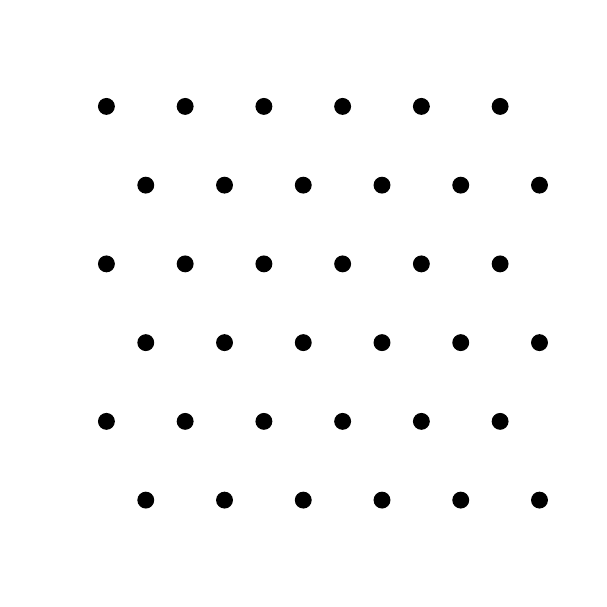
\begin{tikzpicture}
%diamond spacing
\path (0,0) -| (7,7);

\foreach \x in {1,2,...,6}{
\foreach \y in {2,4,6}{
\draw[fill = black] 
(0+\x,0+\y) circle [radius=0.1]
;}}

\foreach \x in {1,2,...,6}{
\foreach \y in {1,3,5}{
\draw[fill = black] 
(0.5+\x,\y) circle [radius=0.1]
;}}

\end{tikzpicture}}

    \caption{Different ways of placing bolts}
    \label{fig:spacebolt}
\end{figure}

Bolt spacing is also an important factor. Diamond spacing is superior at load distribution but square spacing allows for easier installation of mesh with less overlap. \autocite[4.14]{canada96} See \autoref{fig:spacebolt}.
Tight bolt spacing prevents rock ejection. \autocite[217]{Heal10}
%Another important factor is bolt plate size, thickness and surface contact as well interaction between plate and washer. 
The bolt plate is the contact point between reinforcement support and surface support and therefore very important.

\section{Surface Support}
%surface support
One of the functions of surface support, in a dynamic context, is to transfer energy to the reinforcement support. \autocite[210]{Heal10} %In dynamic and purely static use cases surface support has retain broken rock and keep it from falling into the excavation. \autocite[2.16]{canada96} 
Another function is to retain broken rock and to keep it from falling into the excavation. \autocite[2.16]{canada96} Broken rock has be retained both under static stress and during dynamic loading events.

%Surface support elements basic function is to retain broken rock. \autocite[2.16]{canada96} Its secondary function, in a dynamic context, is to transfer energy to the reinforcement support. \autocite[210]{Heal10} 

%Unless lacing, straps or high tensile mesh is used as surface support, the surface support will likely fail before the bolts and at low energy levels. \autocite[240]{Potvin10}
%In \autoref{fig:potsur} the results of several dynamic tests of surface support elements are displayed.

Surface support elements are very diverse. 
Reinforced shotcrete (either with fibres or mesh), welded mesh, chain-link mesh, textile mesh, straps and lacing are typical surface support elements. %Deploying lacing is one way to control large displacements. 
Shotcrete is the stiffest surface support element and most commonly used. \autocite[4.38]{canada96} Shotcrete covers the entire surface of the excavation face and stabilises it. The most common form of shotcrete in use in mining is fibre reinforced shotcrete, FRS. Shotcrete performs well under compressive force, it cracks quickly under tension. It is activated by very small deformations before the rock mass begins to yield. \autocite[578]{sme11} Small surface deformations are therefore contained and spalling is reduced/prevented. \autocite[585]{sme11}
 \autocite[3]{Villa14}. If the stiff support of shotcrete is not necessary a similar effect can be achieved with thin spray on liners TSL. \autocite[22]{guler01} TSL have a thickness of about 5 mm and the technology is not yet fully developed or deployed a large scale. \autocite[591]{sme11}
The are more deformable than shotcrete and can distribute the load on a larger area. \autocite[58]{Guner18}   TSL can be applied directly on the rockmass or on a stabilising a layer of shotcrete. Spraying directly on the rock face is preferable because TSL can infiltrate cracks and gaps and stabilize the rock mass this way. \autocite[113]{archibald92} Some types of TSL hinder the flow of gases. In one trial conducted by \textcite[13]{archibald97} TSL proved 99,8\% effective at stopping the flow of radon. This very low penetrability makes TSL vulnerable to damage by blast gases. \autocite[19]{archibald97}
The reaction forces in TSL under compressive stress are negligible compared to those of the rockmass. Thin layers of shotcrete do not offer a lot of compressive support to the rockmass. If no compressive strength is needed TSL can replace shotcrete. \textcite[99]{komurlu17} stated that a 4 mm layer of TSL can replace a 50 mm layer of shotcrete.
TSL and mesh perform better under tensile strain than shotcrete. \autocite[3]{Villa14}
The use of mesh is necessary in order to connect the surface support to the reinforcement support. In the tests run by \textcite{Heal10} samples without mesh perform significantly worse than those with mesh. As soon as the shotcrete cracks it no longer able to transfer load to individual bolts and if no mesh is used the surface support fails rapidly and the shotcrete turns into fly rock. \autocite[214]{Heal10} \textcite[124]{ansell05} stated that shotcrete reinforced with mesh performs better under dynamic loading conditions than FRS because the mesh stabilises the shotcrete after large cracks have formed. This helps to retain broken rock. Mesh requires significant deformations to be activated. The rock mass likely has at least partially failed by the time these deformations are reached. \textcite[1]{archibald97} stated: '[mesh] often serves no other reinforcement purpose than to prevent rock movement after failure has already occurred.'

Welded mesh is the most common form of mesh. It can easily be used in conjunction with other reinforcement and is very suited for mechanized installation. \autocite[574]{sme11}
% with energy absorption rates (dependant on the reinforcement material) of approximately 1 - 6 \(\rfrac{kJ}{m^2}\) at displacements of < 50 mm. \autocite[4.22]{canada96} Reinforced shotcrete and standard bolts work well together as their survivable displacements tend to be similar. Closed rings of shotcrete can only withstand deformations of 1 \% of the opening diameter. Therefore it can be beneficial to leave strips of exposed mesh between panels of shotcrete, to allow some deformations in order to reduce tensions. 
%Welded mesh is much less stiff than shotcrete, with energy absorption rates (depending on gauge) of approximately 1 - 5 \(\rfrac{kJ}{m^2}\) and maximum displacements of ~ 200 mm. 
%Chain-link is very soft, with very little initial load bearing capacities, it allows for large deformations in the order of 500 mm while absorbing about 7 \(\rfrac{kJ}{m^2}\).\autocite[4.17]{canada96}. 
Chain-link is seldom used as reinforcement for shotcrete because the small openings complicate the application of shotcrete and negatively affect the quality of the finished product. \autocite[344]{Brady99} Chain-link is very flexible and starts to vibrate when shotcrete is applied to it. This vibration causes a lot of rebound and creates waste. (H. Wagner, personal communication, 2019-06-27) 
Chain-link is generally not in wide spread use. \autocite{sme11}. Chain-link mesh has a higher energy absorption capacity than welded mesh. \autocite{Potvin10} \autocite{canada96} \autocite[575]{sme11}
Textile mesh is usually made from synthetic fibres. It can deform more than other mesh types, it is lighter and available in larger rolls. It is also more sensitive to being broken by bolt plates. \autocite[13]{minegrid} It is quite a new development and still has a lot of research potential. 

Straps come in various shapes. For example, mesh straps are strips of strong mesh. Straps can be used in conjunction with with mesh or alone. The are fastened by bolts and used to hold key blocks in place or brace pillars against vertical deformations. \autocite[577]{sme11} 

Lacing also called lace or lashing describes wires or ropes, usually steel, that connect bolts. %in order to distribute local load peaks across a larger area. %Therefore lacing does not increase the support systems load capacity but  %An important factor in the effectiveness of surface support is the strength of the connection to the rock mass and the interlink with neighbouring support elements. 
 \textcite{Ortlepp97} stated: "Lacing is the most important single element in the containment component of a tunnel support system subjected to significant dynamic loading." 
 Lacing connects of individual elements and reduces the load on discrete elements. If a bolt deforms sufficiently, the lacing is activated and transfers load to other bolts down the line. Which means that in case of large displacements, the load on discrete bolts is reduced and the entire support system is activated and energy absorption capacity is greatly increased.\autocite[240]{Potvin10} \autocite[3]{guler01}
 Mesh and straps will most likely buckle under compressive forces and lacing cannot transfer any compressive load. These elements are designed for use in tensile loading situations. \autocite[3]{Villa14}
 %and therefore  increases the energy absorption capacities of the support system. \autocite[240]{Potvin10} \autocite[3]{guler01}
  Lacing has the very large draw back that at the current state of the art, installing it has not been automated and is very labour intensive. \autocite{sme11} Therefore it is not common in countries with high labour costs, like Sweden where Kiirunavaara Mine is located. It was included in the test program because of its potential and just because nobody has automated it yet, does not mean that cannot be done.
 
\textcite{hea09} had different approach to the problem of automating the installation of lacing. A new product was introduced: HEA mesh a hybrid of welded mesh and lacing, that would allow for lacing and mesh to be installed in one step. As of the publications of this thesis, there a no mines using it according to the Australian Centre for Geomechanics. More research in the area might be interesting.

The installation of other surface support elements is easier.
Shotcrete attaches itself directly to the rock mass. TSL does so as well and has the added benefit that the application is automatable \autocite[241]{boeg14}. Different types of mesh and straps needs to be secured somehow. Usually this is one of the bolts secondary functions. In that case the plates of the bolts form the contact point between surface support and reinforcement support. 
Surface support and reinforcement support do not act independently of each other and together they form a support system.

\section{Support System}
%support system

\begin{comment}
\begin{quote}
\textit{    
"The three support elements providing the reinforcement, retaining, and holding functions do not act independently. Therefore, these rock support elements have to be well connected, forming an integrated rock support system."}
\autocite[220]{Kaiser12} \end{quote}

\begin{figure}
    \centering
    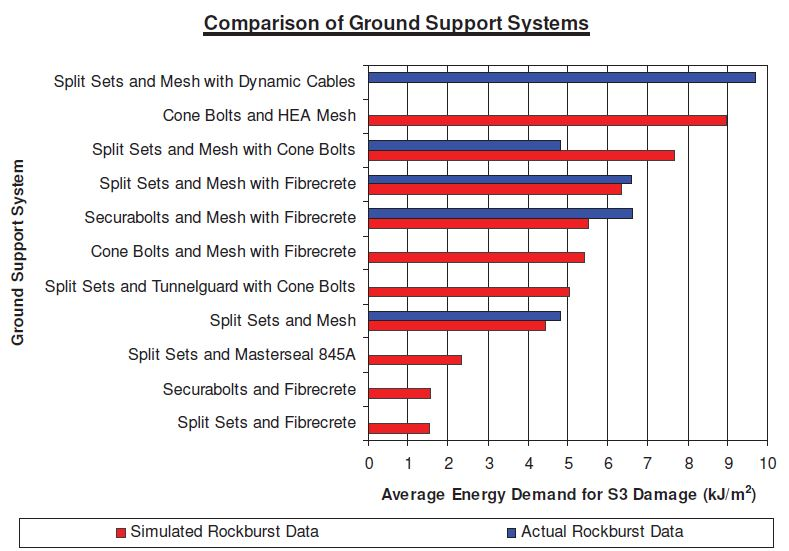
\includegraphics{pics/Heal10.JPG}
    \caption{Comparison of different support systems after \textcite{Heal10}}
    \label{fig:heal10}
\end{figure}
\end{comment}

Reinforcement support, surface support and rock mass form a support system. % that aims to fulfill the previously mentioned support functions. 
As the components work closely together, the support system must be viewed as one unit. There is a lot of interplay between reinforcement and surface support. The energy absorption capacity of a support system is not the sum of the capacity of each individual component. \autocite[1]{Simser07} The capacities for displacement, load and energy absorption must be compatible to ensure the best possible result. \autocite[222]{Kaiser12} 
\textcite[248]{Heal10} stated that: "An ideal integrated ground support system for rockbursting conditions has surface support which is strong enough to transfer load to individual reinforcing elements and engage the full capacity of the rock bolts or cables".
\textcite{Heal10} tested several support systems and evaluated their capacities in real rockbursts. 
%The results are displayed in \autoref{fig:heal10}. The damage level S3 refers to amount of damage a support system can take without rock ejection, which is therefore the level at which the rockburst would not cause any harm to humans present in the area. 
Mesh appears to be necessary to achieve high energy absorption capabilities, without mesh support systems fail at 1,5 - 2 \(\frac{\text{kJ}}{\text{m}^2}\). 
\textcite{Heal10} stated that: "the 1.5 to 2kJ/m\textsuperscript{2} threshold may in fact represents the inherent energy capacity of the unsupported rock mass." which implies that shotcrete alone does not increase the dynamic capabilities of a support system significantly. In order to activate the full potential of the reinforcement support mesh, straps and or lacing are necessary. \autocite[221]{Heal10} 
Shotcrete does stabilise the loose rock around the excavation. For this function a thin layer is enough. \autocite[5]{guler01}
%Lacing increases the energy absorption capabilities of a support system significantly and that chain-link mesh has a higher energy absorption capacity than welded mesh. \autocite{Potvin10} \autocite{canada96} \autocite[575]{sme11}
%Another important factor is bolt plate size, thickness and surface contact as well interaction between plate and washer. 

In burstprone ground a vital task of a support system is dissipating destructive energy, either through deformation, or friction. An important part of a support system are the connections between the different elements. \autocite[2.17]{canada96}\autocite[220]{Kaiser12} A support system will fail when its weakest part fails. Which usually is the reinforcement support. \autocite{Potvin10} \autocite[221]{Kaiser12} 
\autocite[13]{Simser07} If the surface support fails before the reinforcement support, the unbroken bolts remain in the intact rock and are clearly visible. Such a failure mode is called a "naked tendon" failure. \autocite{Potvin10} Such a phenomenon implies the surface support is unable to transfer enough load to the bolts. The loose rock mass detaches itself from bolts during a dynamic event. As the connection between bolt and rock is severed no energy can be transferred, if the surface support does not transfer the energy, the bolts are not loaded. \autocite[7]{guler01} The support system fails at low energy levels, a fraction of its capacity. \autocite[240]{Potvin10}
This is a common phenomenon. Modifying the plates or including straps, lacing or high tensile mesh in the support system can reduce the frequency of this failure mode. \autocite[1]{Simser07} \autocite[240]{Potvin10} 
In order to ensure that the connection between surface support and reinforcement support is strong enough to transfer the impact energy, special attention must be paid to washers, plates and other connective accessories. They should be chosen carefully and thoroughly tested as they often fail in large rockburst events. It´s a known failure mode that bolt nuts simply cut through plates, especially during dynamic events. Thicker and larger plates reduce the frequency of this. \autocite[3]{Simser07}
%An important factor in the effectiveness of surface support is the strength of the connection to the rock mass and the interlink with neighbouring support elements. 
Larger plates help to connect reinforcement support to surface support better.  Welded mesh is susceptible to being damaged by small plates. \autocite[218]{Heal10} Chain-link mesh even more so, as the thinner wires are more easily broken. \autocite{chainlink11}
Another way to handle this is to  put a thin layer of wood or rubber between the plate and the mesh. \autocite[3]{Simser07}
 Lacing is also vulnerable to being damaged by connective elements. It never fails because of rope rupture but instead because the connection elements are the weaker link. \autocite[4.33]{canada96} The strength of lacing therefore is highly dependent on the connective elements (for example: key hole bolts or clamps). If these have sharp edges, lacing ropes might get damaged and fail prematurely. \autocite[3]{guler01} 
%\autocite[221]{Kaiser12} \autocite[129]{chainlink11} Or might damage the surface support. \autocite[218]{Heal10} \autocite[4.33]{canada96} 

Also compatible elements must be chosen to either draw load at the same time or in sequence. For example the maximum deformation of the bolts must fit with the predicted deformation of the rock mass. \autocite[6]{guler01} 

%The sequence of installation of support components is also very important. In order to properly transfer load from the surface support elements to the rock bolts, the bolts must be installed after the surface support elements and with a sufficiently large plates to effectively transfer load. \autocite[4.31]{canada96}

When designing a rock support system in a seismically active mine it is important to keep in mind, what the usual failure modes and their expected severity are and which demands they put on the support system. As well as the constraints put on the support design in order to keep the mine usable. For example what the maximum acceptable displacement is. The rock support system must be able to support the burden of loose rock created through excavation, as well as contain the kinetic energy of ejected rock. It must keep individual rocks from being ejected to protect humans and equipment and finally minimize the inward movement of rock face in total and therefore loss of excavation space. \autocite[4.35]{canada96}
Based on these considerations support elements must be chosen which either are able to prevent the initiation of damage or control the the failure process. \autocite[223]{Kaiser12} 

\textcite[2.8]{canada96} put it this way: 
\begin{quote}\textit{''An ideal support system must either be strong enough to suppress this volume increase or it must have sufficient ductility to allow the volume increase to take place  without destruction of the support system''}
\end{quote} This quote defines the basic approach behind surface support in seismically active mines. Either the support must sufficiently strong to take the load, or it must be flexible enough to deform without destruction. 

In the first case a support system must be strong and provide enough support to keep the rock mass from unravelling. This usually involves using lots of shotcrete. If the demand of the rock on the support system increases, it may not be economically viable to provide the amount of support needed to avoid failure. In this case a different strategy adopted. Soft rock support can be used, which is able to "yield". This means that it has to be able to deform sufficiently to dissipate the energy of an dynamic event. \autocite[220]{Kaiser12} Such a support systems usually include chain-link and lacing. As \textcite[220]{Kaiser12} put it: "A yielding rock support system is a system in harmony with its surrounding, failing rock mass." At the same time, the displacement of the rock support system should be low enough that it is still able to hold the broken rock, produced by the unravelling rock mass, after the seismic event has ended. The larger the displacement the larger the amount of loose rock around the excavation becomes and the more load is put on the surface support.\autocite[7]{villa13} 
After a dynamic event has occurred and the dynamic stresses have dissipated, the static stresses still remain. This means that even after deforming significantly under the dynamic stress
%The support system must retain enough post-peak strength to be able to prevent gravity driven failure of the now loose rock mass after quasi static conditions return. Which means that 
the rock support has to maintain its load carrying capacities. % even after sustaining large deformations. 
\autocite[77]{Heal10}
\textcite[13]{Simser07} advocated a hybrid system of stiff arches and yielding elements in very vulnerable areas.

%"give" under the dynamic load but still be able to function as quasi static support. 
 
%While deformations and associated loss of excavation space are less than ideal they sometimes can not be avoided. %It is acceptable and expected that rock support only survives one large seismic event and needs maintenance afterwards in order to be able withstand the next one.

\section{Factor of Safety}

In order to quantify the likelihood that a given system is going to fail a probability factor can be defined.
Usually this is called the Factor of Safety (FoS) which is defined as displayed in \autoref{equ:FoS} \autocite[3.15]{canada96}.

\begin{equation}
\label{equ:FoS}
FoS = \frac{Capacity}{Demand}
\end{equation}

%\textcite[573]{Masoudi18} states in regard to rockbursts that: 
%"Ground energy demand cannot accurately be determined or calculated." 
%Because the severity and frequency of rock bursts is influenced by several factors, such as: size and geometry of excavation, rockmass properties, \textit{in - situ} stresses and their orientation, distance and energy levels of seismic source, stress wave magnification, support system properties and interplay of these factors. 

The destructive effects caused by different kinds of rockbursts vary strongly, as they are dependant on a number of different factors. The frequency and severity of rockbursts is hard to predict as well. Therefore the demand of the rock mass can not be globally defined. \autocite[8.6]{canada96}
The capacity of rock support must be assessed in terms of energy absorption, displacement and load. \autocite[221]{Kaiser12} 
A support system has to be tailor made for each mine, if not each area of a mine, as local conditions will heavily influence how burst prone the rock mass is. Designing a rock support system is an involved and difficult process that has to deal with ever changing parameters. It has to be adaptable and creative. \autocite[223]{Kaiser12} For this reason \textcite[216]{Kaiser12} described designing a dynamic rock support system as: "interactive and iterative process of selecting proper support elements to form a rock support system which has enough capacity to meet the expected demands" Which means that a design concept has to be modifiable and needs to be adapted to the conditions encountered \textit{in - situ}.

%Usually the reinforcement support is activated by displacement of surface support elements.
%Problems can arise when unyielding bolts are combined with soft surface support, like chain-link mesh. Chain-link requires large displacements before it starts to absorb energy. For example grouted bolts have a displacement limit of 10 - 30 mm, while chain-link mesh´s energy absorbtion capacities are only activated at approximately 100 mm. \autocite[2.20~-~2.22]{canada96} Which means that in this system the reinforcement support has already failed by the time the surface support springs into action. Therefore it is necessary to carefully design support systems in order to maximize synergy.

%''burst control then essentially consists in avoiding or reducing the build-up of such stresses from the beginning'' \autocite[25]{Brauner94} 

\section{Seismic Risk}

Accordingly \textcite{Heal10} suggested a different approach, that takes into account the different needs of different areas of the mine.\textcite{Heal10} coined the term "seismic risk". Seismic risk can be calculated for an arbitrarily small block inside of a mine. It is defined as:
\begin{equation*}
    Seismic~Risk =  Seismic~Hazard * Excavation ~Vulnerability * Exposure
\end{equation*}

The seismic hazard is largely dependent on the expected peak particle velocity PPV. PPV is a function of the distance from the event to the location, as well as the magnitude of an event. The seismic hazard is also influenced by the frequency of seismic events.
The excavation vulnerability depends on the span of the excavation, the deployed ground support system, the ratio of \(\sigma_1\) to the uniaxial compressive strength UCS of the rock mass and the presence of geological structures.
Exposure is defined as the probability of humans being in the area at any given point in time.

As the seismic risk can be calculated for arbitrarily small block of the mine, high risk areas can be identified, and additional measures deployed.